%************************************************
\chapter{Representación de variable discreta}\label{ch:DVR}
% ************************************************
Existen diferentes métodos numéricos para resolver la ecuación de Schrödinger dependiente del tiempo (\autoref{eq:TDSE ket}). En esta capítulo se desarrollará un método particular conocido como el método de \textbf{representación de variable discreta}, \acs{DVR} por sus siglas en inglés.
\\\\
Formalmente, el espacio de Hilbert de las funciones de onda es infinito, sin embargo, para resolver y tratar problemas numéricamente, es necesario hacer un truncamiento de la dimensión del espacio a un número finito $N$. Este espacio reducido de Hilbert, puede verse como un espacio generado por un operador de proyección, además, el espacio reducido de Hilbert tiene el mismo formalismo de la mecánica cuántica, pues, si se recuerda que la dimensión del espacio de Hilbert está dado por las distintas alternativas que puede tomar el sistema cuántico en cuestión, este espacio de dimensión $N$, puede ser un espacio completo para otro problema en mecánica cuántica.

\section{Proyección espectral}
Una función de onda y sus operadores se pueden representar mediante una una base de funciones ortogonales, a esta base se le conoce como \textbf{base espectral}:
$$\{\phi_i(x)\}_{i=1}^{N}$$
que, por ser funciones ortogonales cumplen que:
$$\bra{\phi_i(x)}\ket{\phi_j(x)} = \delta_{ij}$$
Como se mencionó anteriormente, la dimensión del espacio de Hilbert se debe reducir a un número finito $N$, esta reducción de dimensión se puede expresar mediante un \textbf{operador de proyección}:

\begin{equation}
  \label{eq:operadorproyeccion}
  P_N = \sum_{n=1}^N\ket{\phi_n}\bra{\phi_n}
\end{equation}

Mediante el operador $P_N$ se puede mapear la dinámica del espacio de Hilbert al espacio reducido de Hilbert, en particular, es de interés para resolver la \autoref{eq:TDSE ket} conocer cómo se representa el operador Hamiltoniano:
\begin{equation}
  \label{eq:Hamiltoniano}
  H = \frac{\hat{p}^2}{2m}+V(\hat{x})
\end{equation}

Utilizando la base espectral, el Hamiltoniano en el espacio reducido de Hilbert se puede representar como:

\begin{equation}
  \label{eq:Hamiltonianored}
  H_N = P_NHP_N
\end{equation}

Definiendo $Q_N = 1-P_N$, la ecuación de Schrödinger dependiente del tiempo se puede escribir en términos de $P_N$ y $Q_N$ como un conjunto de dos ecuaciones diferenciales acopladas:

\begin{equation}
  \label{eq:acopladas1}
  i\hbar\frac{\partial \psi_N}{\partial t} = P_NHP_N\psi_N + P_NHQ_N\psi_{\perp}
\end{equation}
\begin{equation}
  \label{eq:acopladas2}
  i\hbar\frac{\partial \psi_{\perp}}{\partial t} = Q_NHP_N\psi_N + Q_NHQ_N\psi_{\perp}
\end{equation}


en donde: $\psi_N = P_N\psi$ y $\psi_{\perp}=Q_N\psi$.
\\

Para este trabajo se usará la aproximación de Galerkin \cite{Gottlieb}, en donde se desprecia la contribución de $\psi_{\perp}$, de esta forma, la \acs{TDSE} a resolver es:
\begin{tcolorbox}[colback=CTtitle!5!white,colframe=CTtitle!85!white]%,title=\centering{Ecuación de Schrödinger Dependiente del Tiempo para un estado}]
\begin{equation}
\label{eq:TDSEN}
i\hbar \frac{\partial \psi_N}{\partial t} = P_NHP_N\psi_N
\end{equation}
\end{tcolorbox}

\subsection{Representación de la función de onda}

Una función de onda $\psi(x)$ se puede escribir como una suma infinita en términos de funciones ortonormales $\phi_i$:
\begin{equation}
  \label{eq:wavefuninf}
  \psi(x) = \sum_{n=1}^{\infty}a_n\phi_n(x)
\end{equation}
con:
\[ \int \phi_m^*(x)\phi_n(x)dx = \delta_{mn} \]
\[ a_n = \int \phi_n^*(x)\psi(x)dx\]
para $m,n=1,2,3,\dots, \infty$.
\\
\\
Utilizando la definición del operador de proyección de la \autoref{eq:operadorproyeccion}, se puede probar que:
\begin{equation}
  \label{eq:wavepacketinit}
  \psi_N(x) = P_N\psi(x)=\sum_{n=1}^{N}a_n\phi_n(x)
\end{equation}

\subsection{Colocación del operador de proyección}
Dado un conjunto de puntos en el espacio de posiciones: $\{x_i\}$ con $i=1,2,3,\dots N$, la siguiente relación:
\begin{equation}
  \label{eq:wavefunexp}
  \psi_N(x_i) = P_N\psi(x_i)=\sum_{n=1}^{N}b_n\phi_n(x_i) = \psi(x_i)
\end{equation}

está asociada a la \textbf{colocación}\footnote{Los \textbf{métodos de colocación} son soluciones numéricas de un conjunto de ecuaciones, cuya solución resulta ser exacta en un conjunto discreto de puntos llamados puntos de colocación.\cite{Tannor:2006}} del operador de proyección, y los puntos $\{x_i\}$ son llamados \textbf{puntos de colocación}. Los coeficientes $b_n$ están determinados por la condición de que: $\psi_N(x)=\psi(x)$ en el conjunto de puntos de colocación.


\section{Base pseudo-espectral}
Una \textbf{base pseudo-espectral}: $\{\theta_j\}_{j=1}^N$ se define como la base de las funciones localizadas espacialmente. La base de funciones ortogonales $\{\phi_n\}_{n=1}^N$, la colocación en la \autoref{eq:wavefunexp}, los puntos de colocación $\{x_i\}_{i=1}^N$, y los factores de peso definidos como $\Delta_j$ con $j=1,\dots,N$, determinan completamente la forma de la base pseudo-espectral:

\begin{equation}
  \label{eq:basepseudo}
  \theta_j(x) \equiv \sum_{n=1}^N\phi_n(x)\Phi_n^*(x_j)
\end{equation}
donde:
$$\Phi_n(x_j)\equiv \sqrt{\Delta_j}\phi_n(x_j)$$
$$\theta_j(x_i) = \Delta_j^{-1/2}\delta_{ij}$$


En conjunto, las $N$ funciones de la base pseudo-espectral generan el mismo espacio de Hilbert reducido que las $N$ funciones ortogonales de la base espectral, y ambas bases están relacionadas mediante una transformación unitaria: $\Phi_n^*$. Como consecuencia, se tiene que el operador de proyección es idéntico en ambas bases, es decir:
\begin{equation}
  \label{eq:proyecbases}
  P_N = \sum_{n=1}^N\ket{\phi_n}\bra{\phi_n}=\sum_{j=1}^N\ket{\theta_j}\bra{\theta_j}
\end{equation}

Se puede probar \cite{Tannor:2006}, que tanto la base espectral, como la base pseudo-espectral tienen propiedades de completes y ortogonalidad completamente análogas. Esto es de particular importancia, pues, dado que ambas bases generan el mismo espacio reducido de Hilbert, los operadores se pueden escribir tanto en términos de una base, como en la otra, y, si es necesario hacer cálculos con estos operadores (como sumarlos), se puede utilizar la transformación unitaria para escribirlos en términos de la misma base.


\section{Algoritmo DVR aplicado a un proceso físico-químico}\label{sec:DVRapp}

En esta sección se aplicarán los conceptos revisados a lo largo del capítulo para resolver un problema físico-químico que involucra potenciales dependientes del tiempo utilizando el método \acs{DVR}.\\
La implementación numérica se realizó en Python 3.9.7 y se encuentra disponible en el repositorio: \href{https://github.com/Jessi-MM/PropagatorLearning/blob/main/src/ANN_as_Propagators_DidacticNotebook.ipynb}{\faGithub Transferencia de Protones}

\subsection{Sistema de transferencia de protones}\label{sec:ProtonTransfer}

Los sistemas de \textbf{transferencia de protones} ocurren en un complejo de enlaces de hidrógeno: $A-H\dotsb A'$. El modelo simplificado se muestra en la siguiente figura:

\begin{figure}[ht]
  \centering
\includegraphics[width=0.6\textwidth]{/home/jessica/Tesis/img/DrawModel.png}
\caption{Descripción del modelo de transferencia de protones $H^+$.}
\label{fig:drawmodel}
\end{figure}

En donde la coordenada $Q$ hace referencia a la separación entre los átomos $A$ y $A'$, mientras que la coordenada $r$ es la distancia del protón al centro de los enlaces. \cite{DynamicalTheoryPTS}. \\
En las descripciones teóricas de la transferencia de protones, a menudo el hidrógeno es representado moviéndose a través de un pozo de doble potencial unidimensional. \cite{Enzymes}
\\

A continuación se presenta un modelo particular de potencial para el sistema de transferencia de protones, en donde la descripción está dada por la coordenada del protón $r \in [-1.5 \,\,\mathring{A}, 1.5 \,\,\mathring{A}]$. A cada tiempo $t$ el valor del potencial $V(r,t)$ está dado por el eigenvalor más bajo de la siguiente matriz:

\begin{equation}
  \label{eq:matrixPot}
  \begin{pmatrix}
    U_1(r,R(t)) &   V \\
    V           & U_2(r,R(t))+X(t)
  \end{pmatrix}
\end{equation}

En donde $U_1(r,R(t))$ y  $U_1(r,R(t))$ son potenciales de oscilador armónico, y $V$ es una constante.

\begin{equation}
  \label{eq:U1}
  U_1(r,R(t))=\frac{1}{2}m\omega_1^2\left( r + \frac{R(t)}{2} \right)
\end{equation}

\begin{equation}
  \label{eq:U2}
  U_2(r,R(t))=\frac{1}{2}m\omega_2^2\left( r - \frac{R(t)}{2} \right)
\end{equation}

En las ecuaciones de potenciales de oscilador armónico, $m$ se refiere a la masa del protón, $\omega$ es la frecuencia del pozo de protones. Los términos $U_1(r,R(t))$ y  $U_1(r,R(t))$ están desplazados mediante un término de energía dependiente del tiempo: $X(t)$, y un termino de distancia dependiente del tiempo: $R(t)$. La dinámica de $X(t)$ corresponde a las fluctuaciones del entorno, mientras que $R(t)$ representa las vibraciones de los sitios donantes y aceptores de protones. \cite{Main:2021}

\begin{equation}
  \label{eq:X(t)}
  X(t)=\lambda \cos(\omega_xt+\theta_x)+X_{eq}
\end{equation}

\begin{equation}
  \label{eq:R(t)}
  R(t)=(R_0-R_{eq})\cos(\omega_Rt + \theta_R) + R_{eq}
\end{equation}

\begin{figure}[ht]
  \centering
  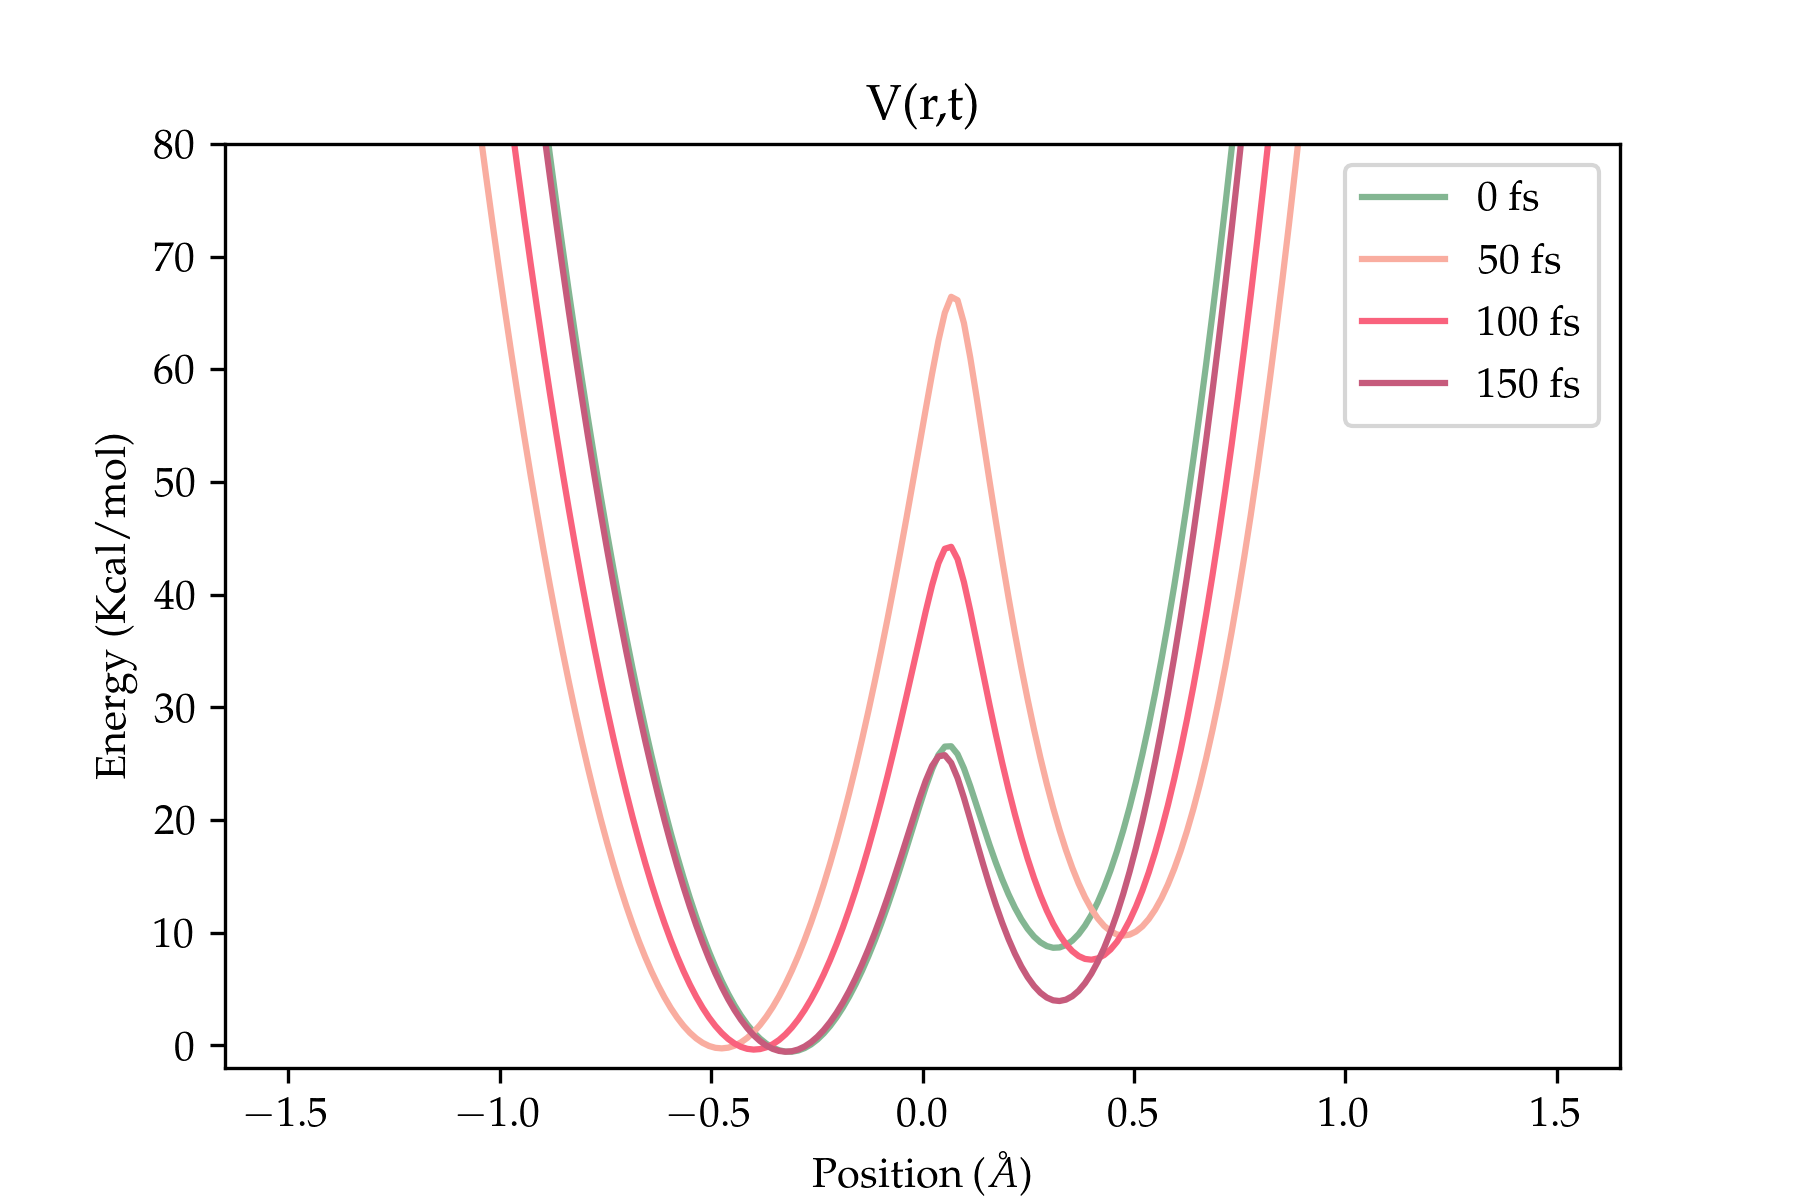
\includegraphics[width=1\textwidth]{/home/jessica/Tesis/img/tesis/ExamplesPotential1.png}
  \caption{Potencial $V(r,t)$ a diferentes tiempos.}
  \label{fig:drawPot}
\end{figure}

La \autoref{fig:drawPot} muestra un ejemplo de potencial $V(r,t)$ generado con la implementación de las ecuaciones anteriores. Los parámetros de potencial utilizados se muestran en la \autoref{tab:ValuesPlot1}

\subsection{Elección de una base ortonormal y grid}

Para proceder con la solución a la \acs{TDSE} \autoref{eq:TDSE ket}, elegimos una base de funciones ortogonales: \cite{Colbert1992}

\begin{equation}
  \label{eq:eigenfunc}
  \phi_n(r)=\sqrt{\frac{2}{b-a}}\sin\left( \frac{n\pi(r-a)}{b-a}\right) \,\,\,\,\, n=1,..,N
\end{equation}

y un grid en el espacio de posiciones:
\begin{equation}
  \label{eq:grid}
  r_i = a + \frac{(b-a)i}{N-1} \,\,\,\,\, i=0,..,N-1
\end{equation}

donde: $a=-1.5\AA$, $b=1.5\AA$ y $N=200$ para la implementación numérica, es decir, que el espacio reducido de Hilbert del sistema tiene una dimensión de $N=200$. La \autoref{fig:Phi_n} muestra las primeras cinco funciones ortogonales de la base en el grid del espacio de posiciones. Las funciones $\phi_n$ están construidas para que se cumpla: $\phi_n(r=r_0=a)=\phi_n(r=r_{N-1}=b)=0$.

\begin{figure}[ht]
  \centering
  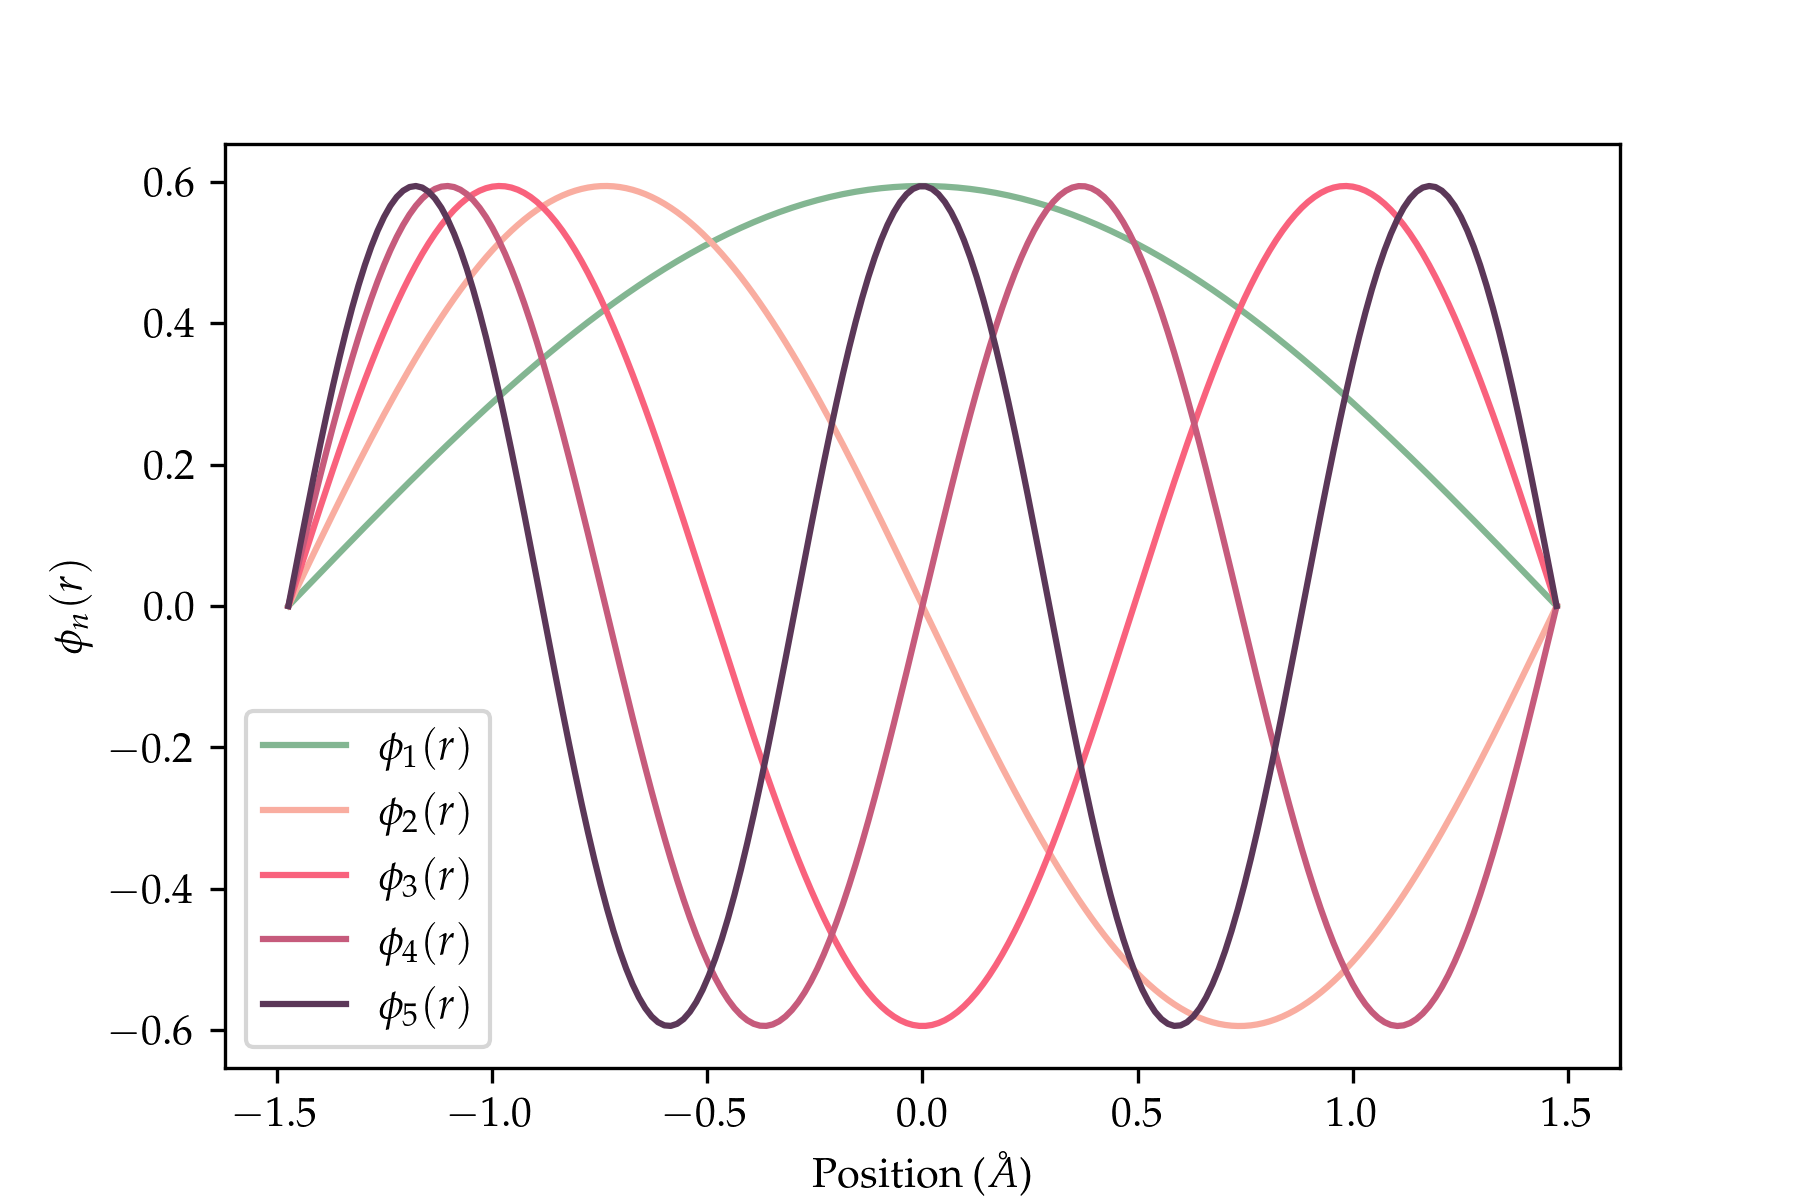
\includegraphics[width=1\textwidth]{/home/jessica/Tesis/img/tesis/Phi_n1.png}
  \caption{Funciones ortogonales $\phi_n(r)$ en el grid $\{r_i\}_{i=0}^{N-1}$ para $n=1,..5$.}
  \label{fig:Phi_n}
\end{figure}

\subsubsection{Representación de la matriz del Hamiltoniano en la base espectral}

Los elementos de matriz de la energía cinética en la base pseudo-espectral están dados por:
\begin{equation}
  \label{eq:T}
T^{\theta}_{ij}= \bra{\theta_i}T\ket{\theta_j}=\sum_{n=1}^N\bra{\theta_i}\ket{\phi_n}\bra{\phi_n}T\ket{\theta_j}
\end{equation}
realizando la aproximación:
$$\bra{\theta_j}T\ket{\phi_n} \approx \bra{r_j}T\ket{\phi_n}$$
y considerando que el operador $T$ en el espacio de posiciones $r$ está dado por:
\begin{equation}
  \label{eq:Toperator}
  T = -\frac{\hbar^2}{2m}\frac{d^2}{dr^2}
\end{equation}


se puede obtener que: \cite{Tannor:2006}\cite{Colbert1992}
\begin{equation}
  \label{eq:T_DVR}
  T^{\theta}_{ij}\approx -\frac{\hbar^2}{2m}\Delta r\sum_{n=1}^{N}\phi_n(r_i)\frac{\partial^2\phi_n}{\partial r^2}\biggr\rvert_{r_j}
\end{equation}

donde: $\Delta r = (b-a)/N-1$. Obteniendo la segunda derivada de la \autoref{eq:eigenfunc}, y sustituyendo en la \autoref{eq:T_DVR} se tiene:

\begin{equation}
  \label{eq:T_N}
  T^{\theta}_{ij}=\frac{\hbar^2}{2m}\left(\frac{\pi}{b-a} \right)^2\frac{2}{N-1}\sum_{n=1}^Nn^2\sin\left(\frac{n\pi i}{N-1} \right)\sin\left(\frac{n\pi j}{N-1} \right)
\end{equation}

que son los elementos de matriz de la energía cinética en la base pseudo-espectral, $T^{\theta}\in \mathcal{M}_{200\times200}(\mathbb{R})$.
\\
\\
La representación de la matriz de energía potencial en la base pseudo-espectral es más simple que la de la energía cinética, pues 
las funciones $\{\theta_i\}$ son localizadas en el espacio de posiciones $r$ y cumplen la condición de ortogonalidad: $\bra{\theta_i}\ket{\theta_j}= \delta_{ij}$, así:

\begin{equation}
  \label{eq:V_DVR}
  V^{\theta}_{ij}= \bra{\theta_i}V(\hat{r})\ket{\theta_j}=V(r_i)\delta_{ij}
\end{equation}

$V^{\theta}\in \mathcal{M}_{200\times200}(\mathbb{R})$ es una matriz diagonal.
\\
Dado un tiempo $t$, los elementos de la diagonal $V^{\theta}_{ii}$ están dados por $V(r_i,t)$ (\autoref{eq:matrixPot}), con $i=0,..,199$.
\\
A partir de la \autoref{eq:T_N} y \autoref{eq:V_DVR}, se construye la matriz del Hamiltoniano en la base pseudo-espectral al tiempo $t$:
\begin{equation}
  \label{eq:H_DVR}
  H(t)^{\theta} = V(t)^{\theta}+T^{\theta}
\end{equation}
en donde el Hamiltoniano tiene dependencia temporal debido a que el potencial del sistema es dependiente del tiempo.

\subsection{Propagación de un paquete de onda}

Sea un paquete de onda al tiempo $t=0$ (\autoref{fig:psi_0}): 
\begin{equation}
  \label{eq:psi_0}
\psi(r,0)=\sum_{i=1}^{k=5}C_i \cdot \phi_{i}(r)
\end{equation}
con $C_i$ números complejos aleatorios de una distribución uniforme, y elegidos de tal forma que: $\bra{\psi(r,0)}\ket{\psi(r,0)}=1$
\begin{figure}[!htbp]
  \centering
  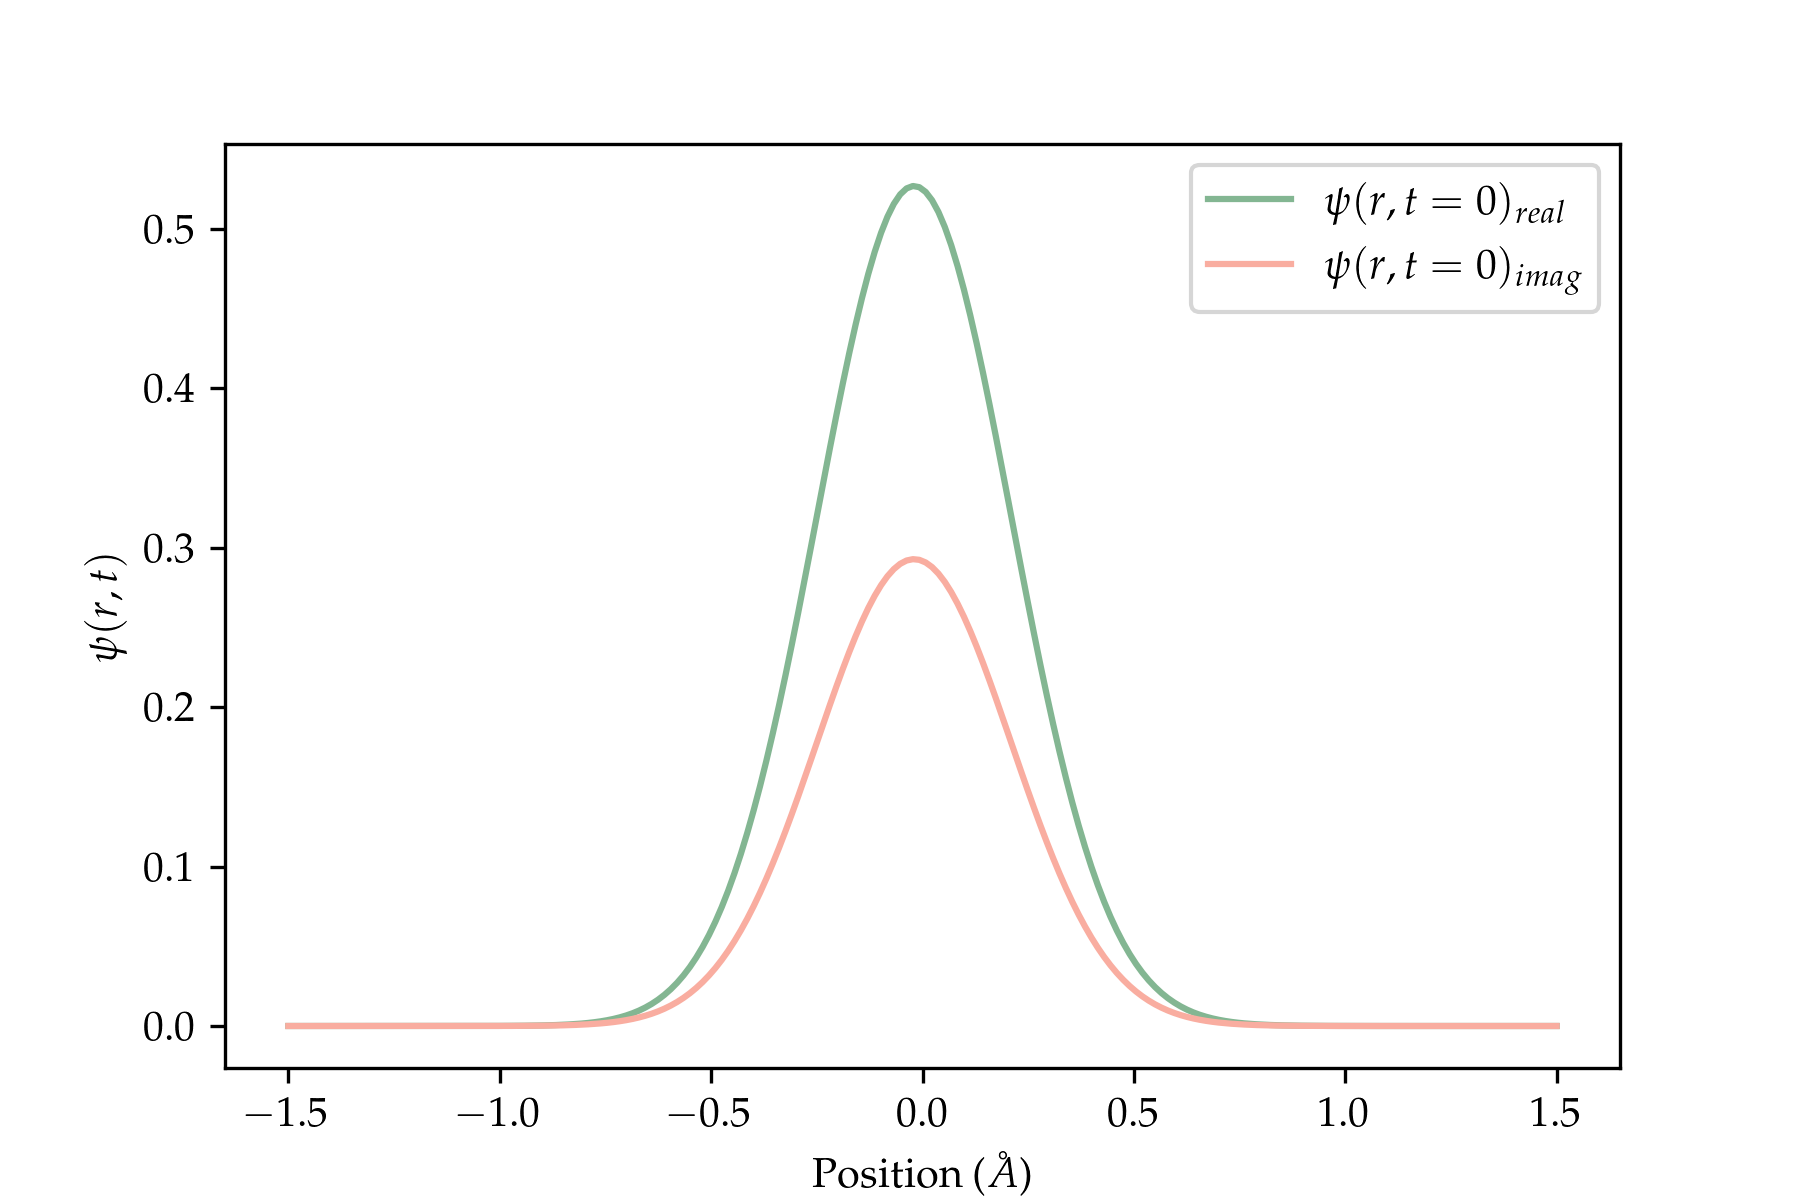
\includegraphics[width=0.9\textwidth]{/home/jessica/Tesis/img/tesis/psi_01}
  \caption{Paquete inicial de onda al tiempo $t=0$. Parte real y compleja.}
  \label{fig:psi_0}
\end{figure}

Si se toma un intervalo de tiempo $\Delta t$ lo suficientemente pequeño como para que el potencial se pueda considerar constante en ese intervalo de tiempo ($\approx 1\,\,fs$ para el sistema en cuestión), la evolución temporal del paquete de onda está dado por (\autoref{eq:U IT}):
\begin{equation}
  \label{eq:wp_ev}
  \psi(r,t)=\exp{-iH^{\theta}t/\hbar}\psi(r,0)
\end{equation}

Si $H^{\theta} = UDU^{-1}$, con $D$ una matriz diagonal:
$$ \psi(r,t) = \exp{-iUDU^{-1}t/\hbar}\psi(r,0)$$  
así,
\begin{equation}
  \label{eq:psi_t}
\psi(r,t) = U\exp{\frac{-it}{\hbar}D}U^{-1}\psi(r,0)
\end{equation}

En donde la matriz $U$ está formada por los $N$ eigenvectores de $H^{\theta}$ como vectores columna, y:
$$D=U^{-1}H^{\theta}U$$
\\

La \autoref{fig:psi_evre} y la \autoref{fig:psi_evim} muestran la evolución de la parte real e imaginaria del paquete de onda en intervalos de $1\,fs$ a lo largo de $20\,fs$, obtenidas con la \autoref{eq:psi_t}. En la \autoref{fig:dens_ev} se muestra la evolución temporal de la densidad del protón.\\
\href{https://github.com/Jessi-MM/PropagatorLearning/blob/main/src/Animacion/gifs/animation-dens\%26pot.gif}{\faPlayCircle[regular] Evolución Temporal: Potencial y Densidad}

\begin{figure}[!htbp]
  \centering
  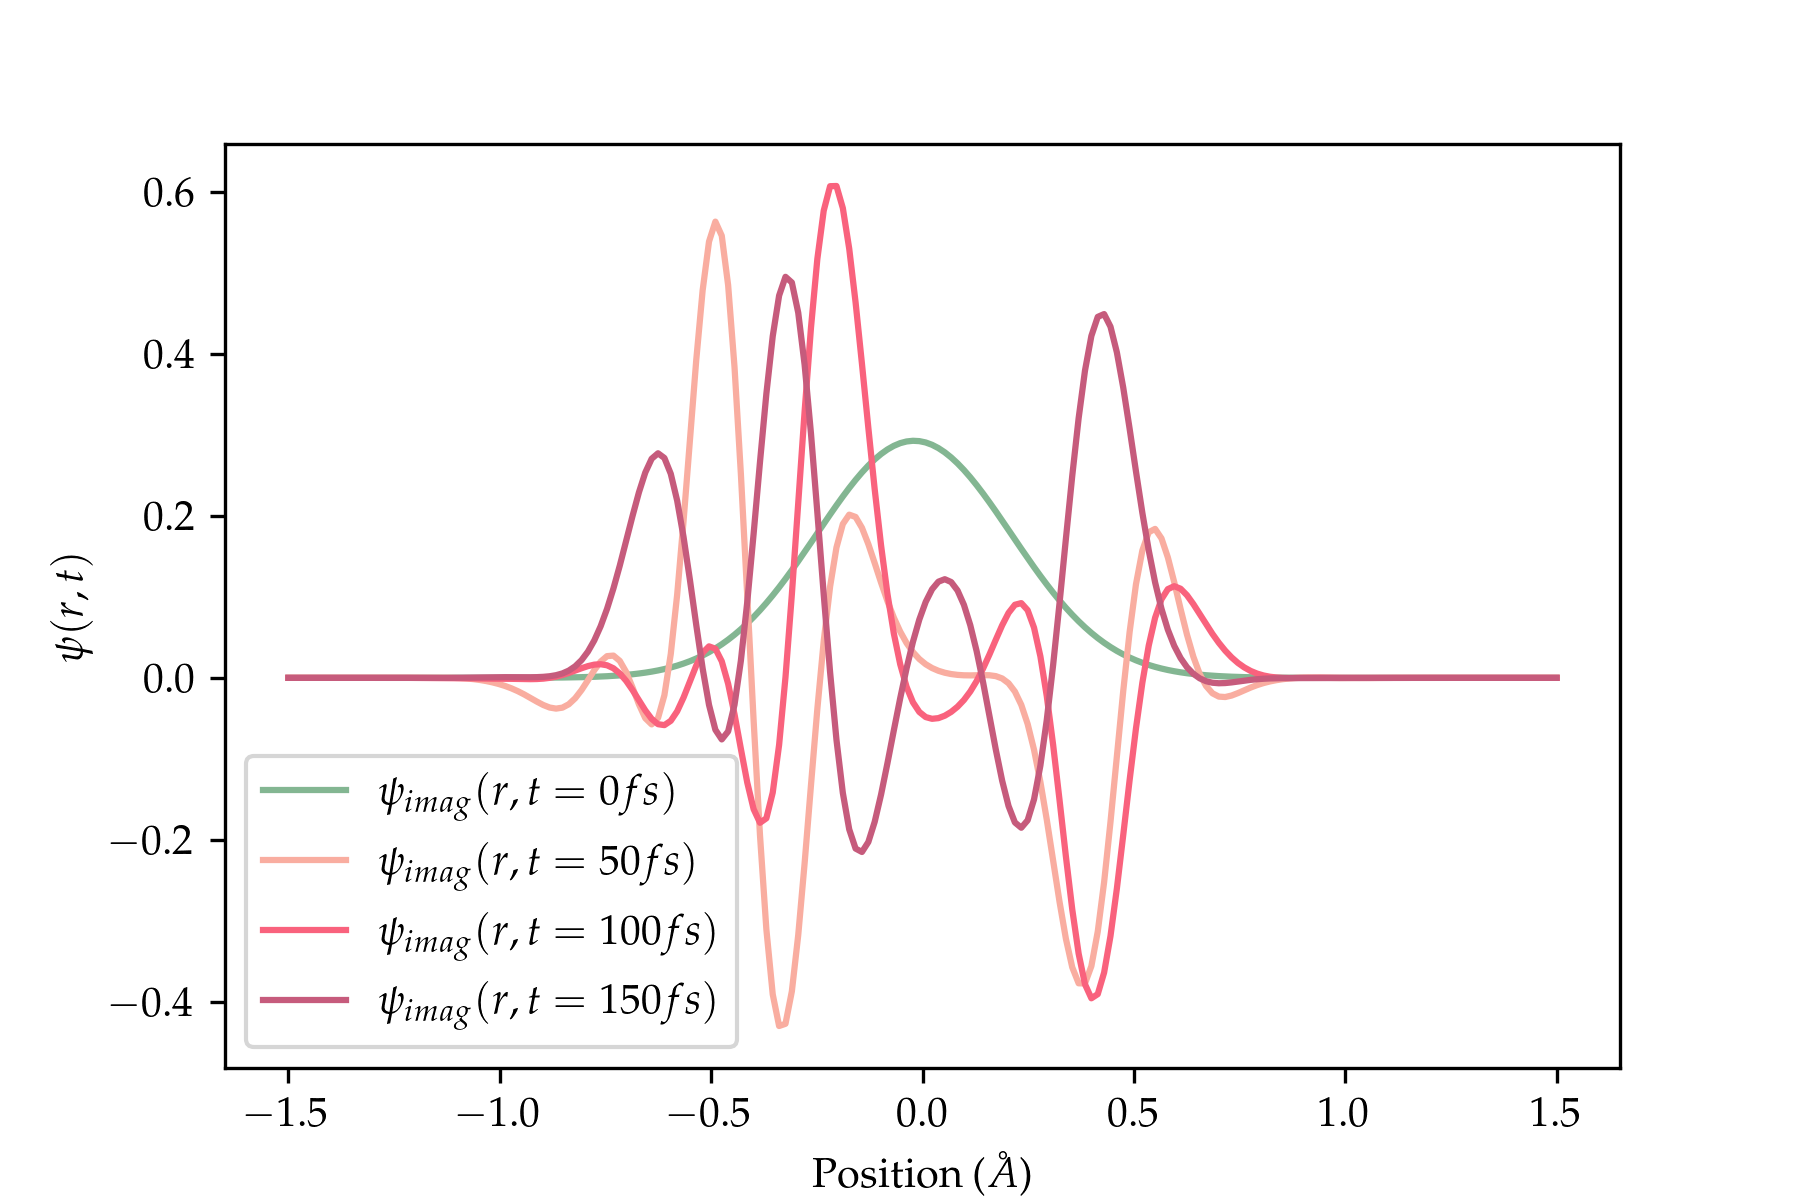
\includegraphics[width=1\textwidth]{/home/jessica/Tesis/img/tesis/psi_ev1real}
  \caption{Propagación del paquete de onda $\psi(r,t)$ parte real.}
  \label{fig:psi_evre}
\end{figure}

\begin{figure}[!htbp]
  \centering
  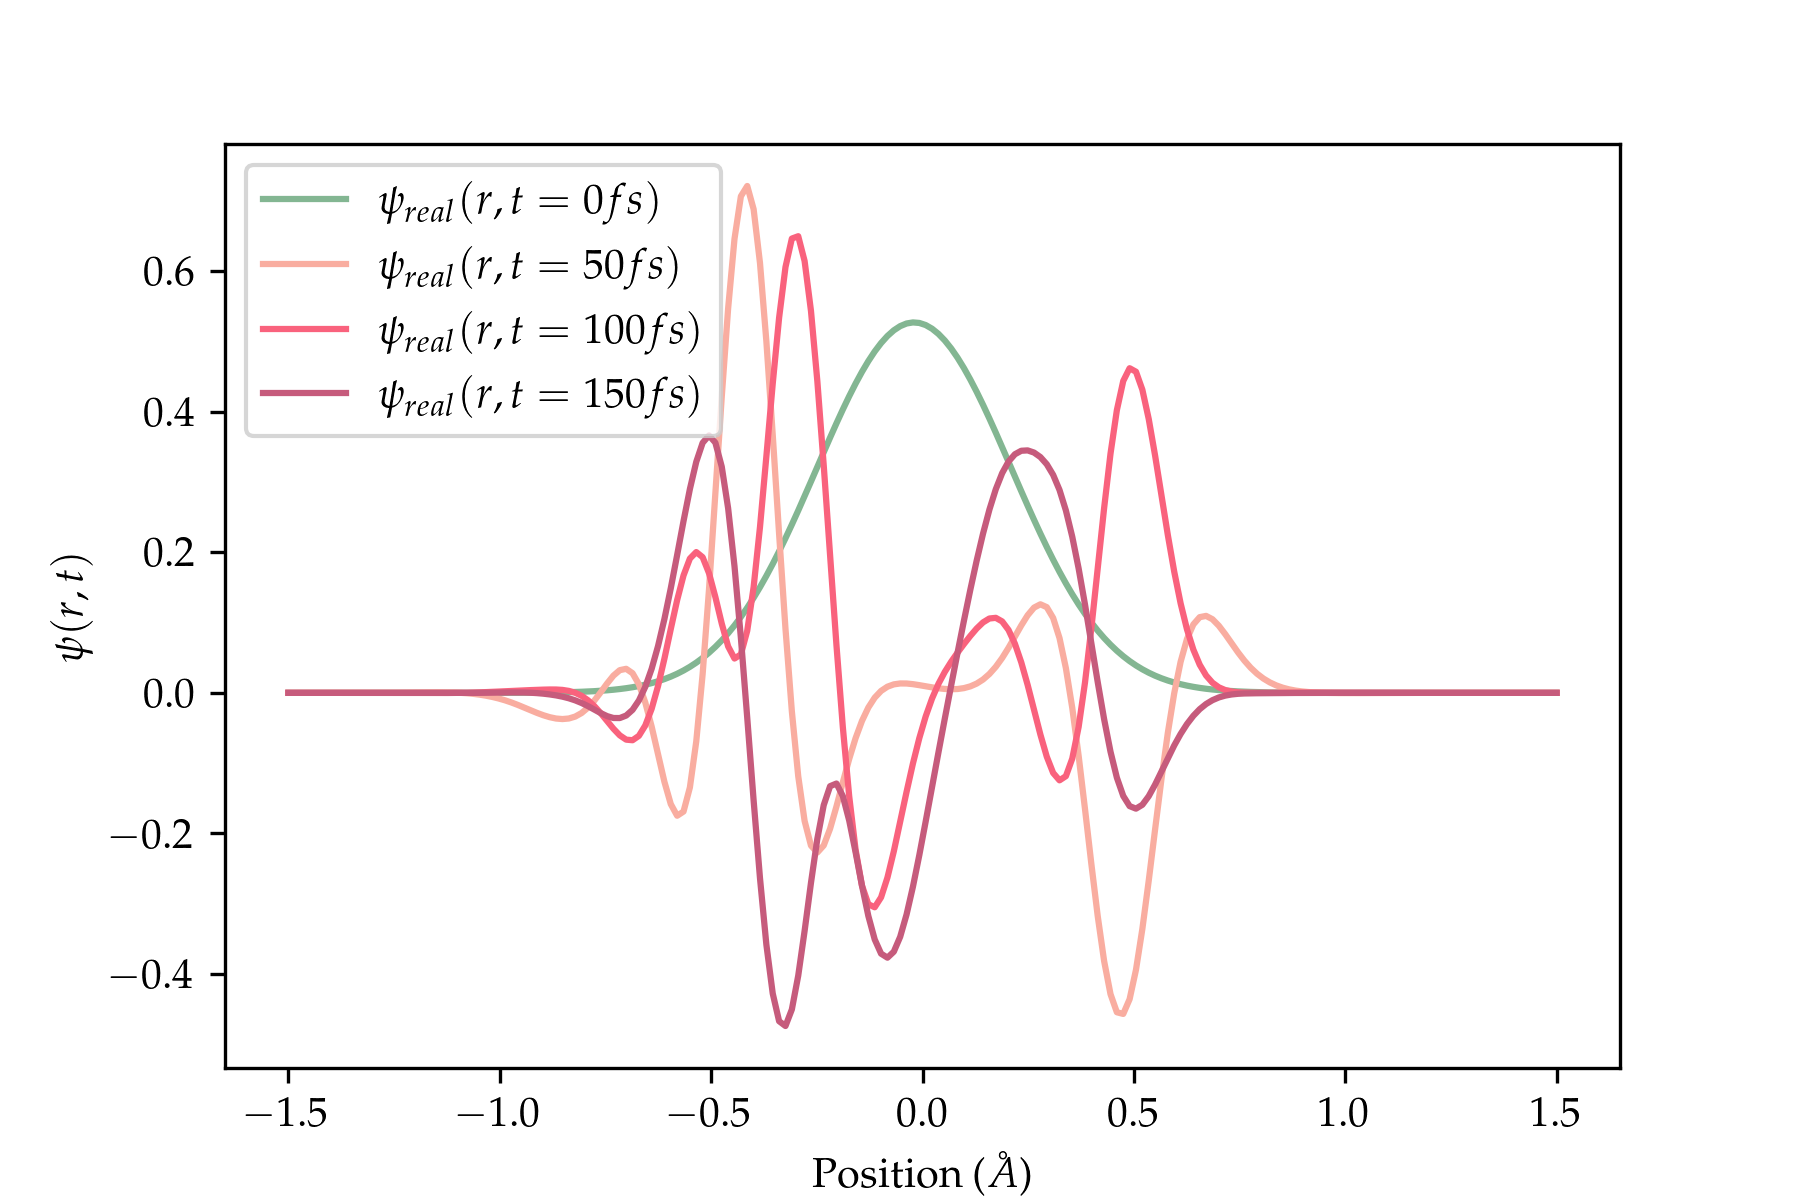
\includegraphics[width=1\textwidth]{/home/jessica/Tesis/img/tesis/psi_ev1imag}
  \caption{Propagación del paquete de onda $\psi(r,t)$ parte imaginaria.}
  \label{fig:psi_evim}
\end{figure}

\begin{figure}[!htbp]
  \centering
  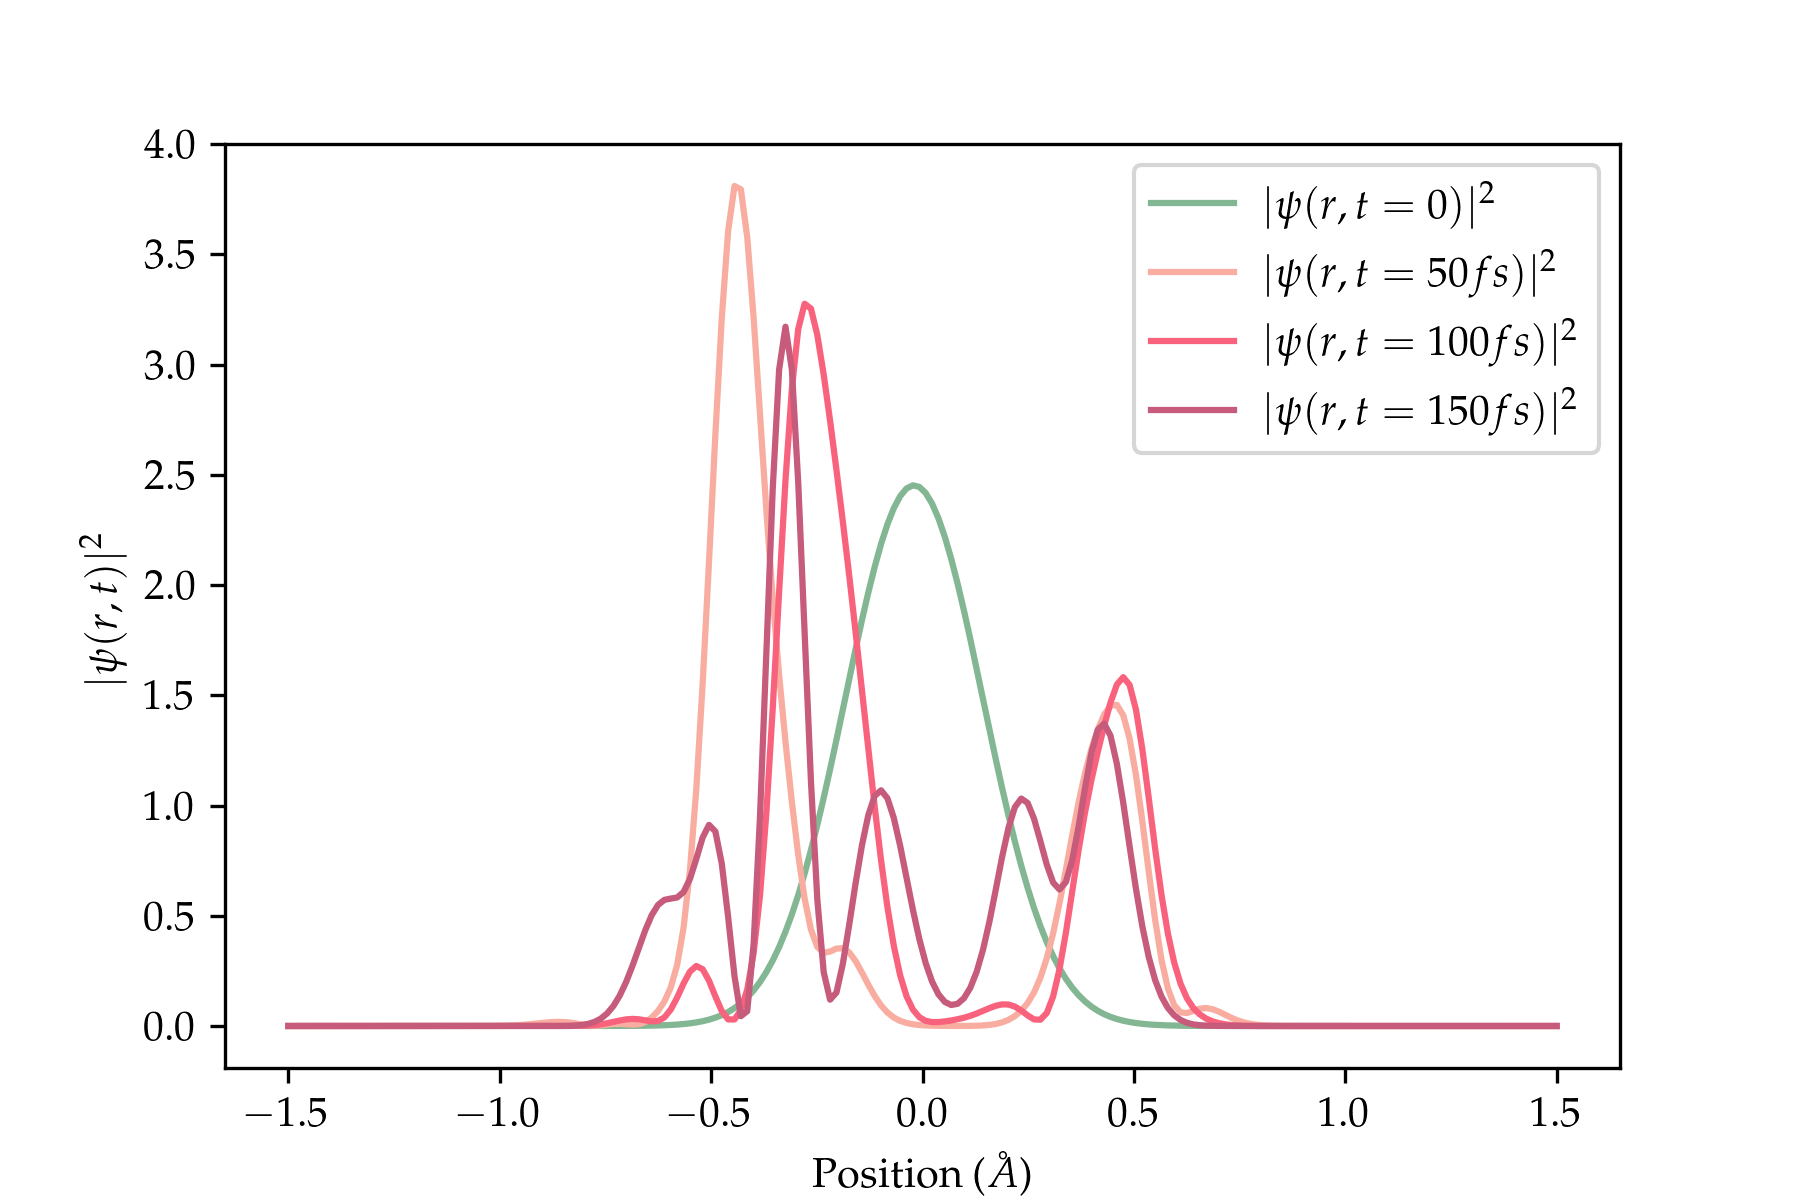
\includegraphics[width=1\textwidth]{/home/jessica/Tesis/img/tesis/dens_ev1}
  \caption{Evolución temporal de la densidad $|\psi(r,t)|^2$.}
  \label{fig:dens_ev}
\end{figure}
